%% Overleaf			
%% Software Manual and Technical Document Template	
%% 									
%% This provides an example of a software manual created in Overleaf.

\documentclass{ol-softwaremanual}

% Packages used in this example
\usepackage{graphicx}  % for including images
\usepackage{microtype} % for typographical enhancements
\usepackage{hyperref}  % for hyperlinks
\usepackage[a4paper,top=4.2cm,bottom=4.2cm,left=3.5cm,right=3.5cm]{geometry} % for setting page size and margins
\usepackage[spanish,es-tabla]{babel}
\selectlanguage{spanish}
% Custom macros used in this example document
\newcommand{\doclink}[2]{\href{#1}{#2}\footnote{\url{#1}}}
\newcommand{\cs}[1]{\texttt{\textbackslash #1}}
\graphicspath{ {./img/} }
% Frontmatter data; appears on title page
\title{Manual de usuario}
\version{1.0}
\author{Teodoro Ricardo García Sánchez}
\softwarelogo{
\includegraphics[width=8cm]{logo}}

\begin{document}

\maketitle

\tableofcontents

\newpage

\section{Introducción}

``Prompt sentiment'' es una aplicación que realiza un análisis de sentimientos sobre un 
fichero que contiene una serie de reseñas de usuario relacionadas con un producto o servicio.\\
Esta aplicación utiliza OpenAI para analizar las reseñas mediante técnicas de ``prompt engineering''.
En un futuro próximo se ampliará el soporte con otros modelos LLM como Llama o Mistral.

\newpage
\section{Registro}
Para empezar a utilizar la aplicación lo primero que nos hace falta es crear un usuario.
Empiece accediendo a la página de registro: \href{https://promptsentiment.es/registro}{https://promptsentiment.es/registro}.

\vspace{25pt}
\centerline{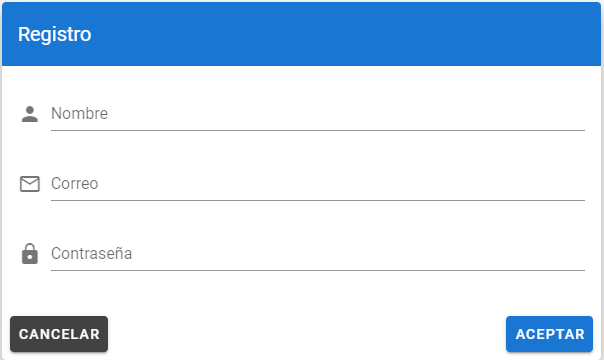
\includegraphics[width=8cm]{es/registro.png}}
\vspace{25pt}

Si falta algún dato o es incorrecto (por ejemplo, el formato de correo no es correcto), se mostrará un mensaje de error.

\vspace{20pt}
\centerline{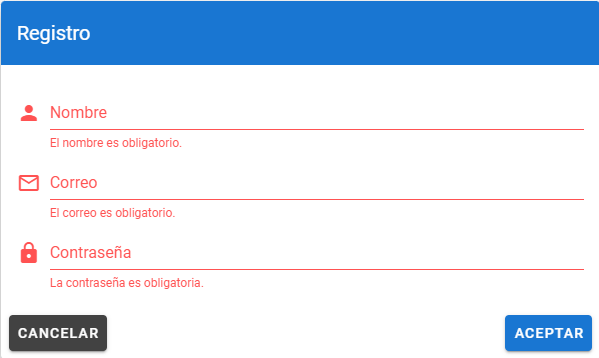
\includegraphics[width=8cm]{es/registro_error.png}}
\vspace{20pt}

NOTA: El perfil asignado al nuevo usuario creado es el de Gestor. Éste es un perfil limitado. Contacte con el administrador 
de la aplicación para actualizar su perfil a otro más avanzado.
\newpage
\section{Login}

Un vez se ha registrado correctamente en la aplicación aparecerá la pantalla de login.\\

\vspace{20pt}
\centerline{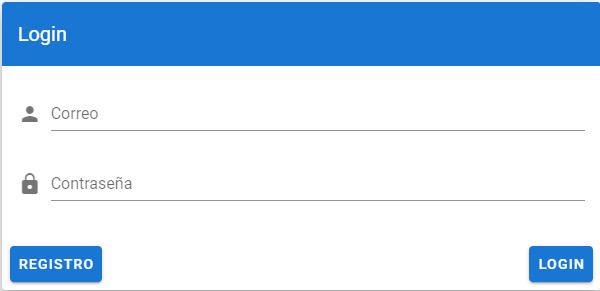
\includegraphics[width=8cm]{es/login.png}} 
\vspace{20pt}

Si falta algún dato o es incorrecto (por ejemplo, el formato de correo no es correcto), se mostrará un mensaje de error.\\

\vspace{20pt}
\centerline{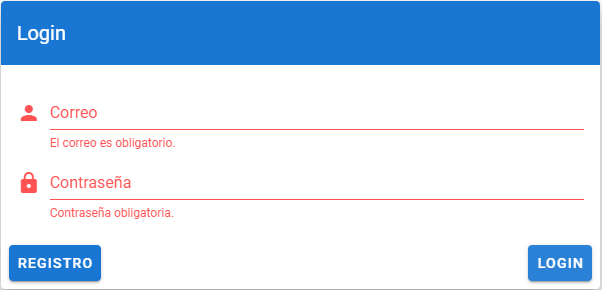
\includegraphics[width=8cm]{es/login_error1.png}}
\vspace{20pt}

Si el usuario no existe o la contraseña es incorrecta se mostrará un mensaje de error.

\vspace{20pt}
\centerline{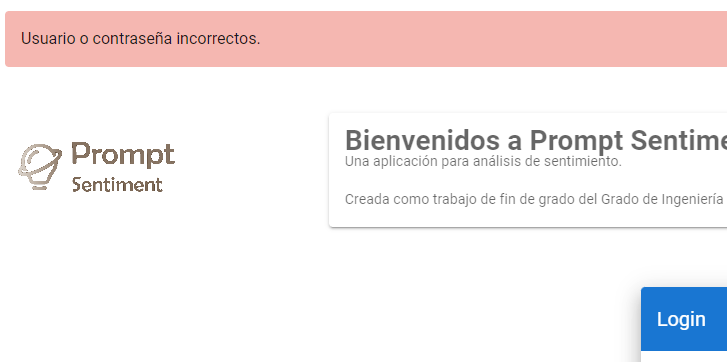
\includegraphics[width=8cm]{es/login_error2.png}}
\vspace{20pt}

\newpage
\section{Inicio}
Una vez hecho login correctamente en la aplicación aparecerá la pantalla de inicio.\\
En la pantalla de inicio hay 2 opciones que se pueden seleccionar:
\begin{itemize}
    \item Análisis de reseñas
    \item Histórico de reseñas
\end{itemize}

\vspace{20pt}
\centerline{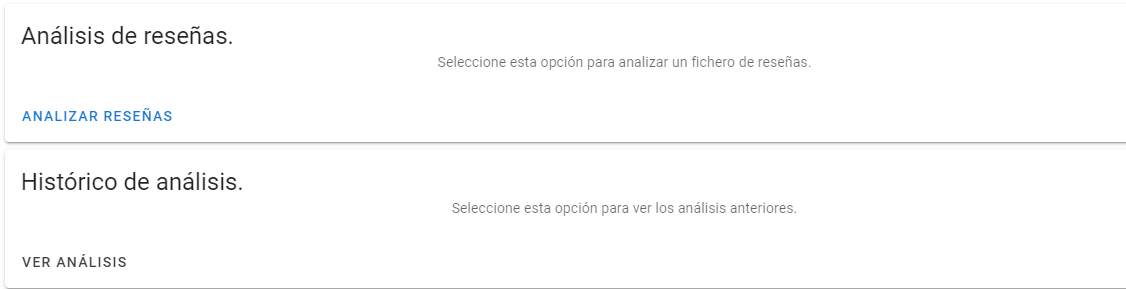
\includegraphics[width=14cm]{es/inicio.png}}
\vspace{20pt}

También se puede cambiar el idioma del interfaz.

\vspace{20pt}
\centerline{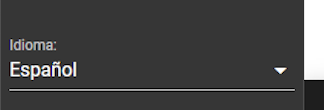
\includegraphics[width=8cm]{es/language1.png}}
\vspace{20pt}

Y acceder al menú de la aplicación y activar el modo oscuro.

\vspace{20pt}
\centerline{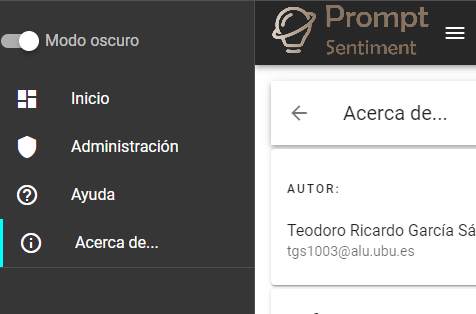
\includegraphics[width=8cm]{es/menu.png}}
\vspace{20pt}


\newpage
\section{Análisis de reseñas}
El análisis de reseñas se realiza en 3 pasos:

\begin{itemize}
    \item Paso 1: selección del fichero de reseñas
    
    \vspace{20pt}
    \centerline{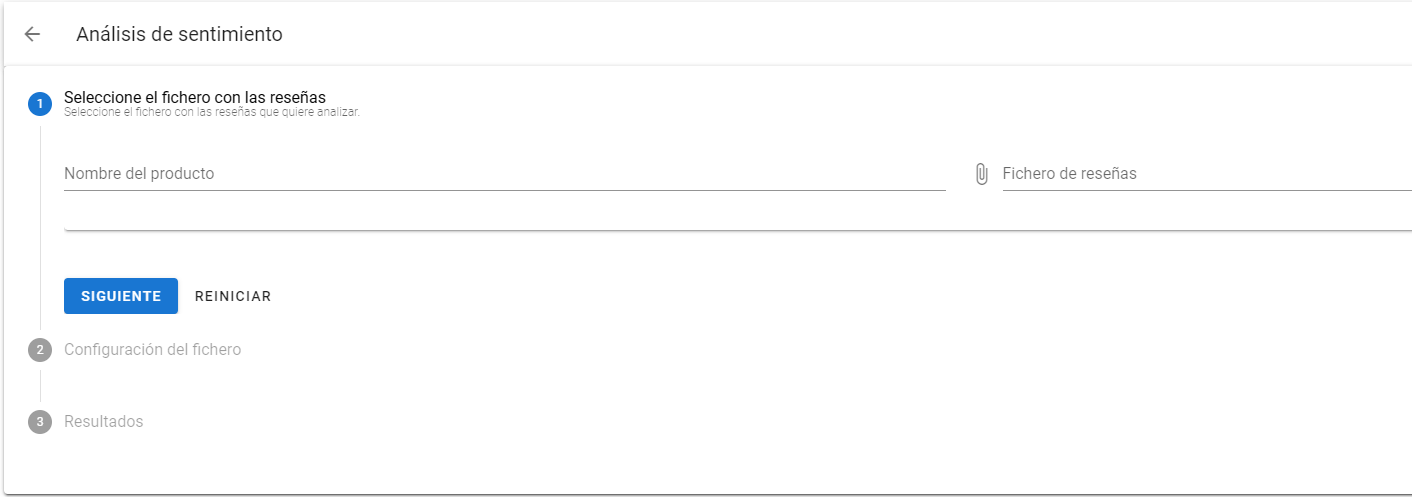
\includegraphics[width=10cm]{es/analisis_paso1.png}}
    \vspace{20pt}

    \item Paso 2: configuración del formato del fichero
    
    \vspace{20pt}
    \centerline{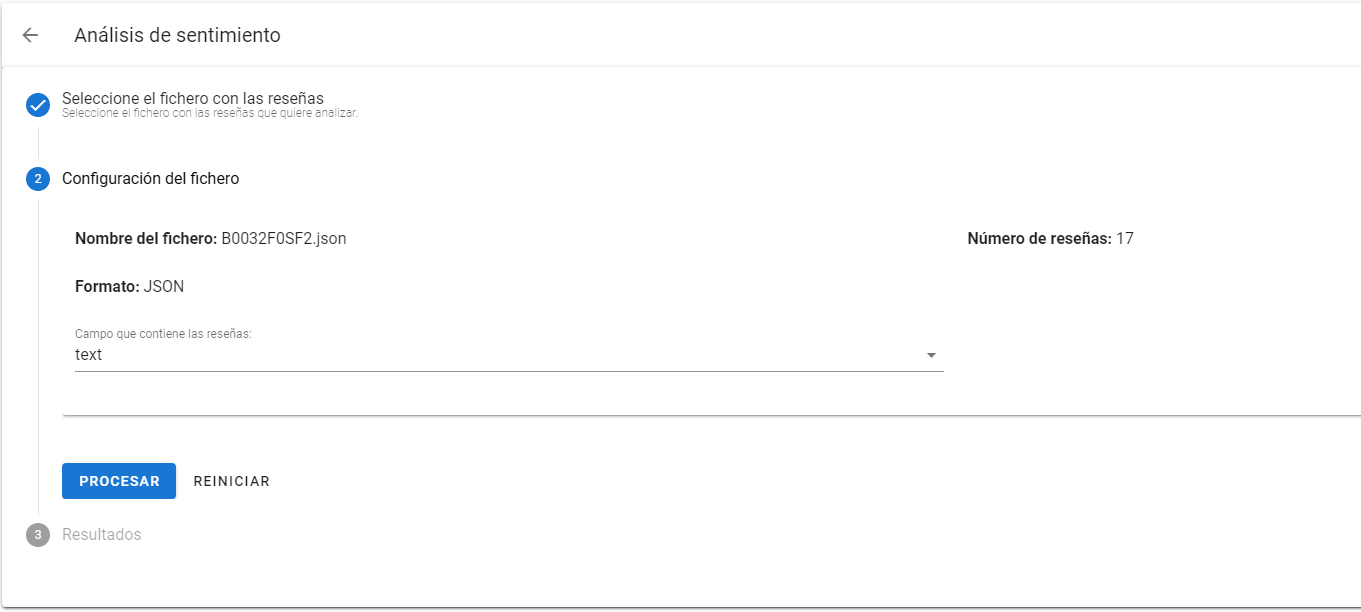
\includegraphics[width=10cm]{es/analisis_paso2.png}}
    \vspace{20pt}

    \item Paso 3: importar y procesar las reseñas
    
    \vspace{20pt}
    \centerline{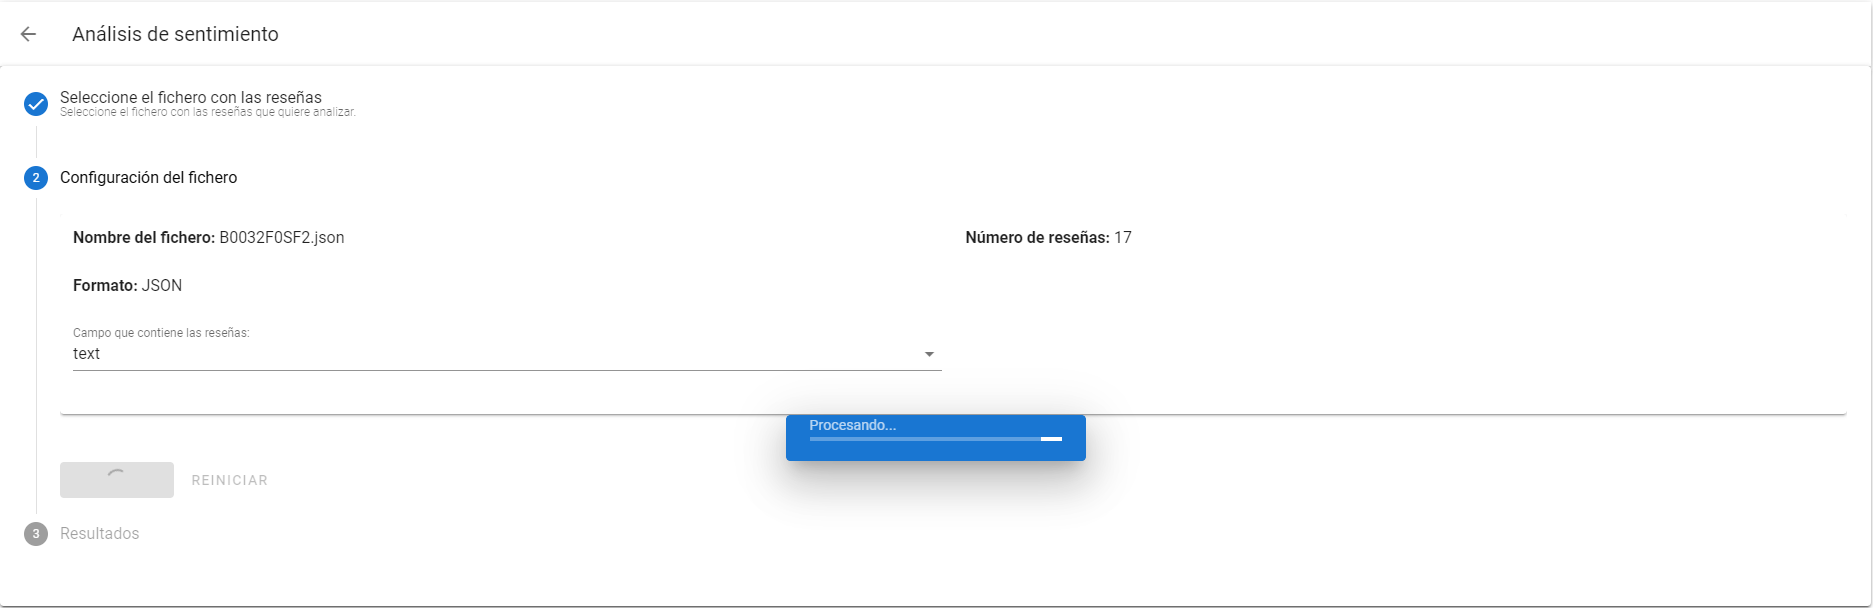
\includegraphics[width=10cm]{es/analisis_paso2bis.png}}
    \vspace{20pt}
\end{itemize}

\newpage

Una vez terminado el proceso obtenemos los resultados:

\vspace{20pt}
\centerline{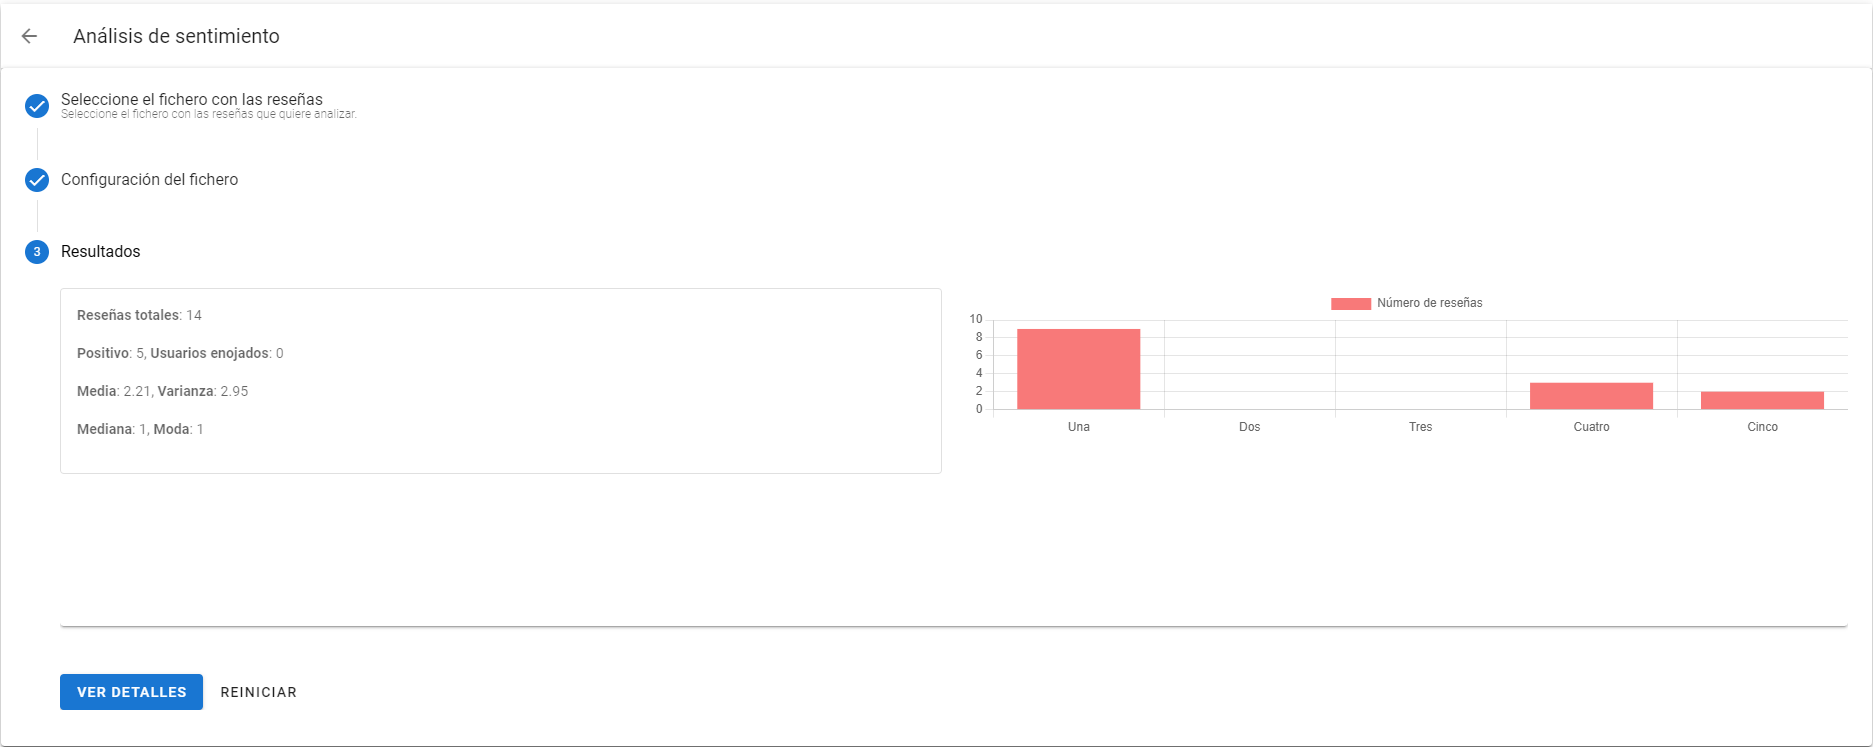
\includegraphics[width=10cm]{es/analisis_paso3.png}}
\vspace{20pt}

También podemos ver los resultados detallados:

\vspace{20pt}
\centerline{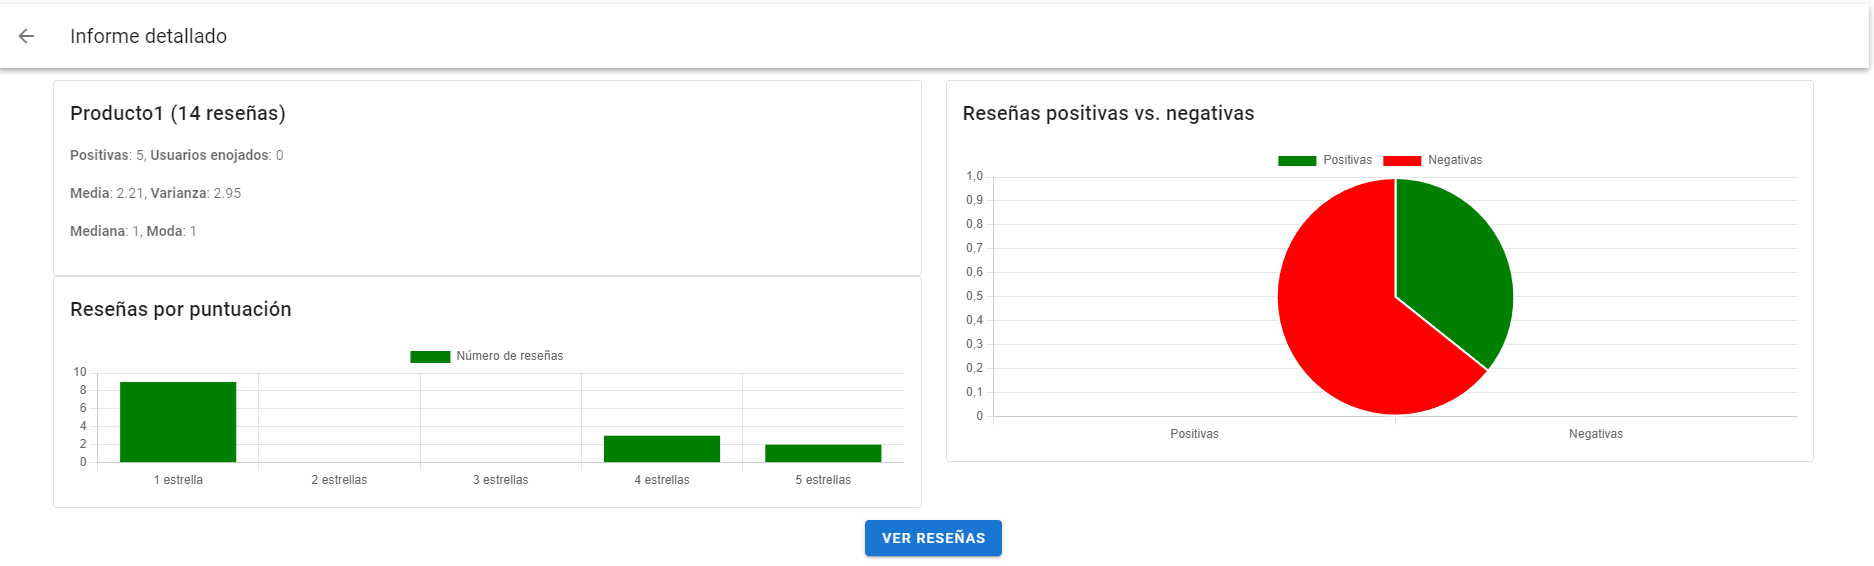
\includegraphics[width=10cm]{es/informe_detallado.png}}
\vspace{20pt}

Y ver las reseñas desde esa pantalla:

\vspace{20pt}
\centerline{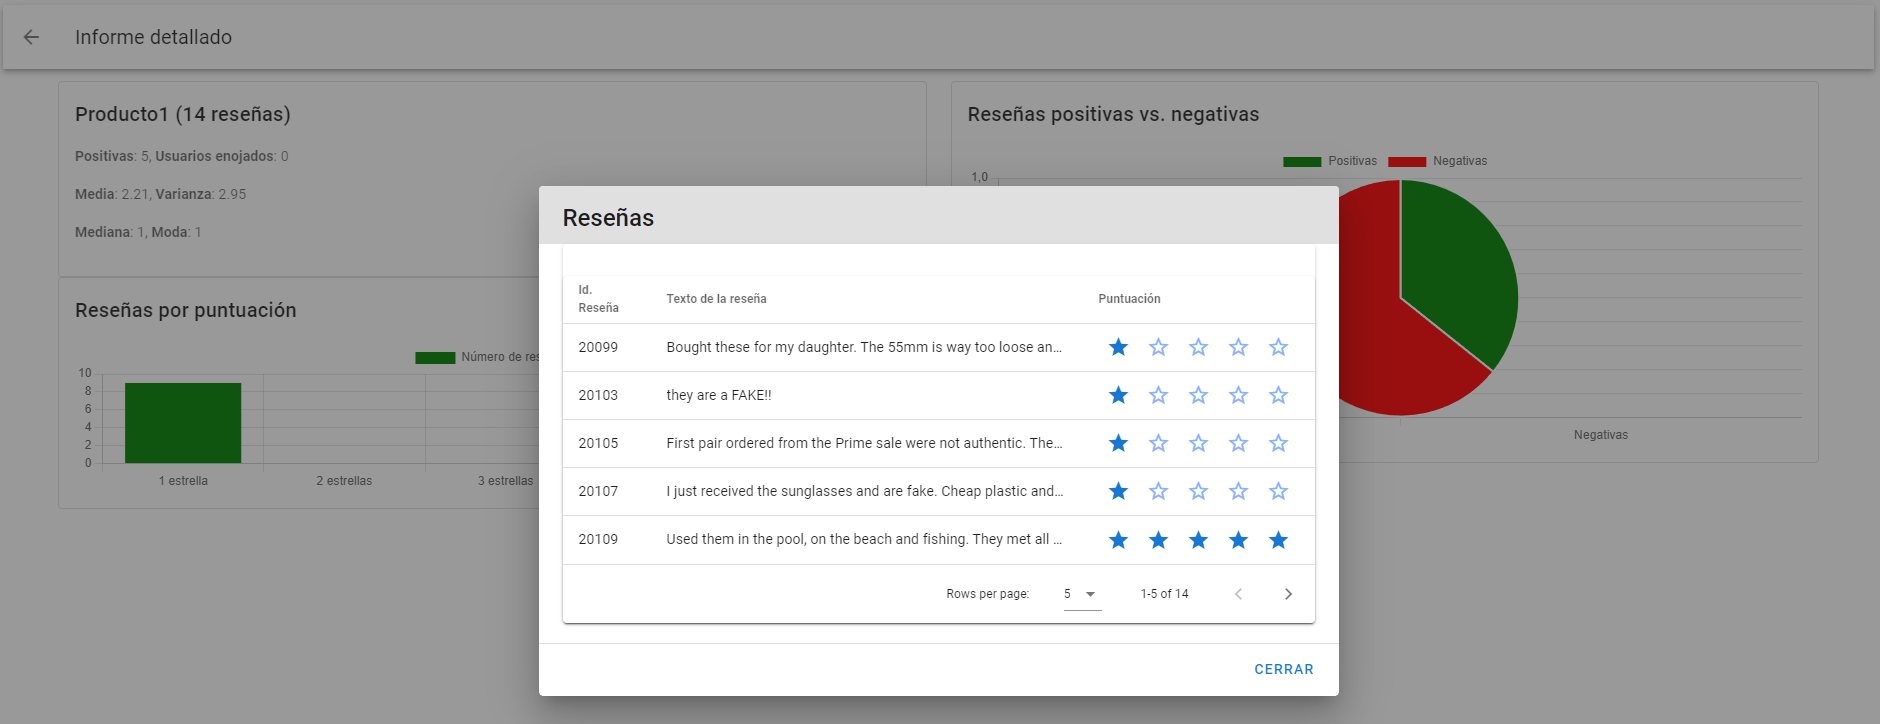
\includegraphics[width=8cm]{es/informe_detallado_resenas.png}}
\vspace{20pt}

\newpage
\section{Histórico de reseñas}
Desde la página de inicio también podemos acceder al histórico de reseñas. En el histórico podemos ver los ficheros de reseñas analizados en la aplicación.

\vspace{20pt}
\centerline{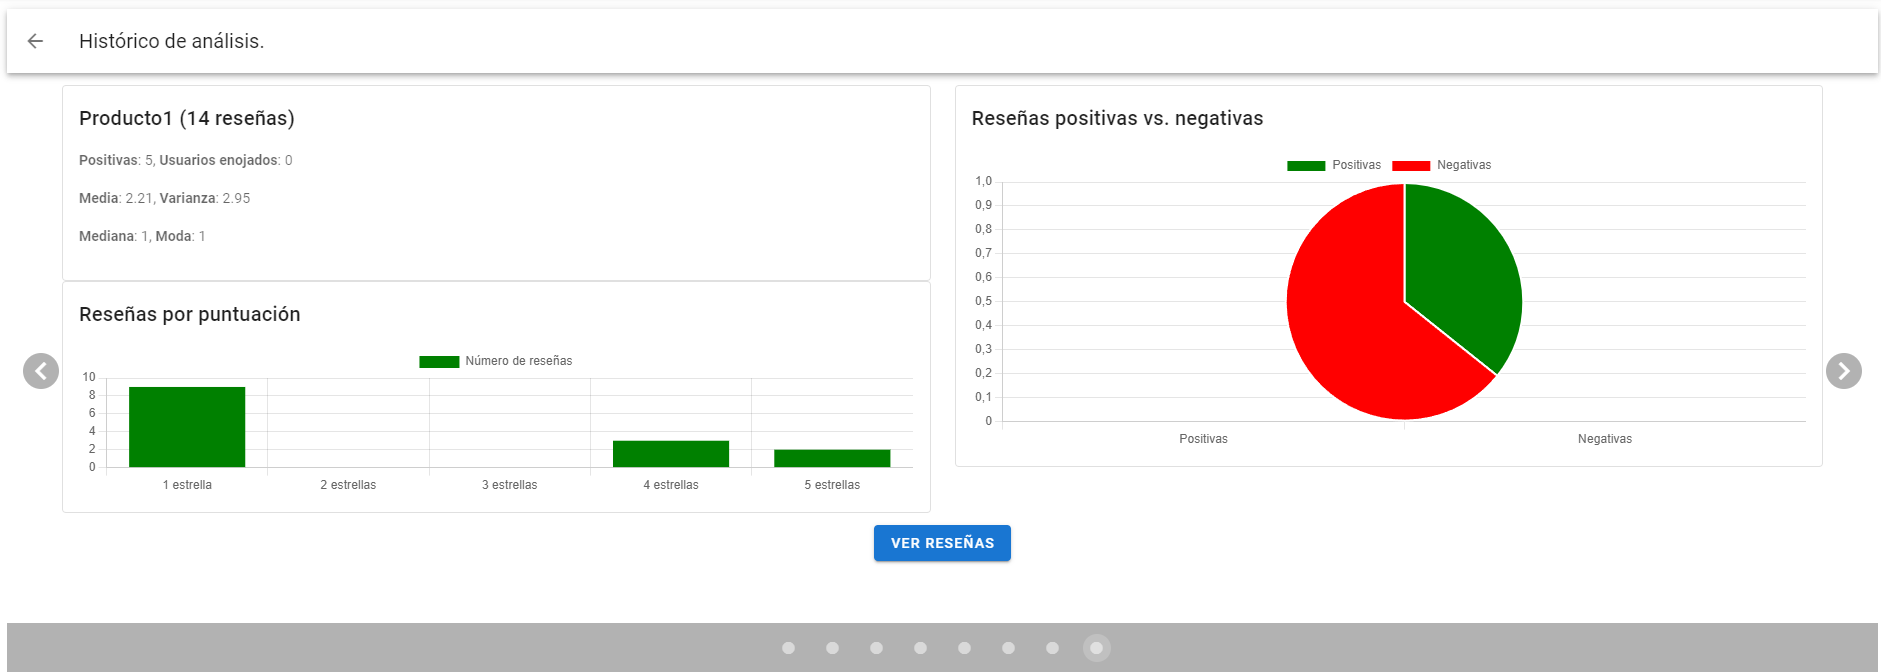
\includegraphics[width=10cm]{es/historico.png}}
\vspace{20pt}

También podemos ver las reseñas desde esta pantalla:

\vspace{20pt}
\centerline{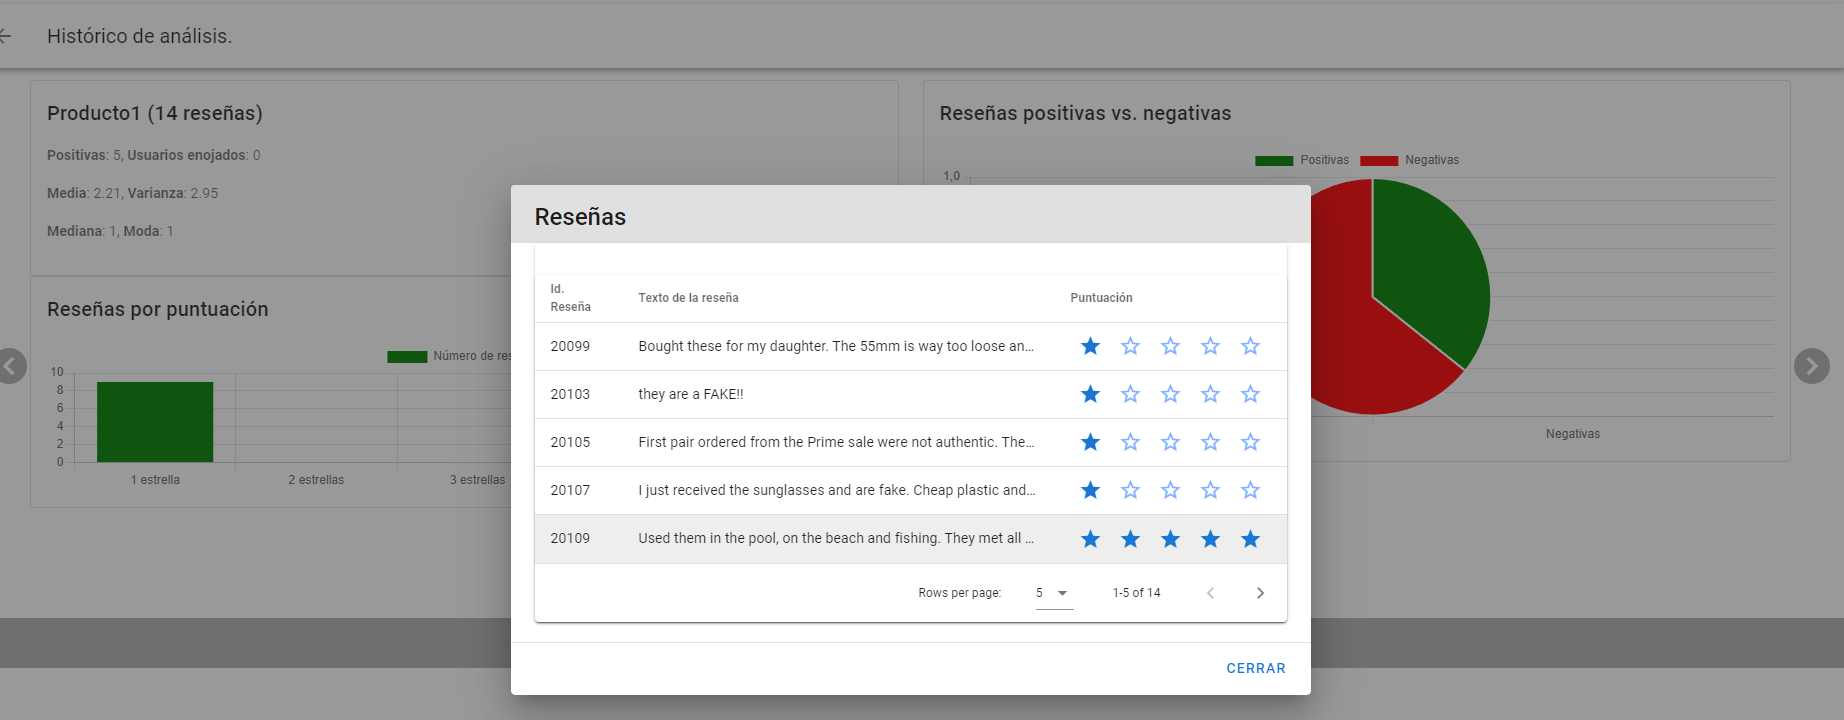
\includegraphics[width=10cm]{es/historico_resenas.png}}
\vspace{20pt}

\newpage

\section{Administración}
La pantalla de administración es sólo accesible para usuarios con perfil de administración (Admin).

Desde esta pantalla podemos administrar usuarios y conjuntos de datos:
\vspace{20pt}
\centerline{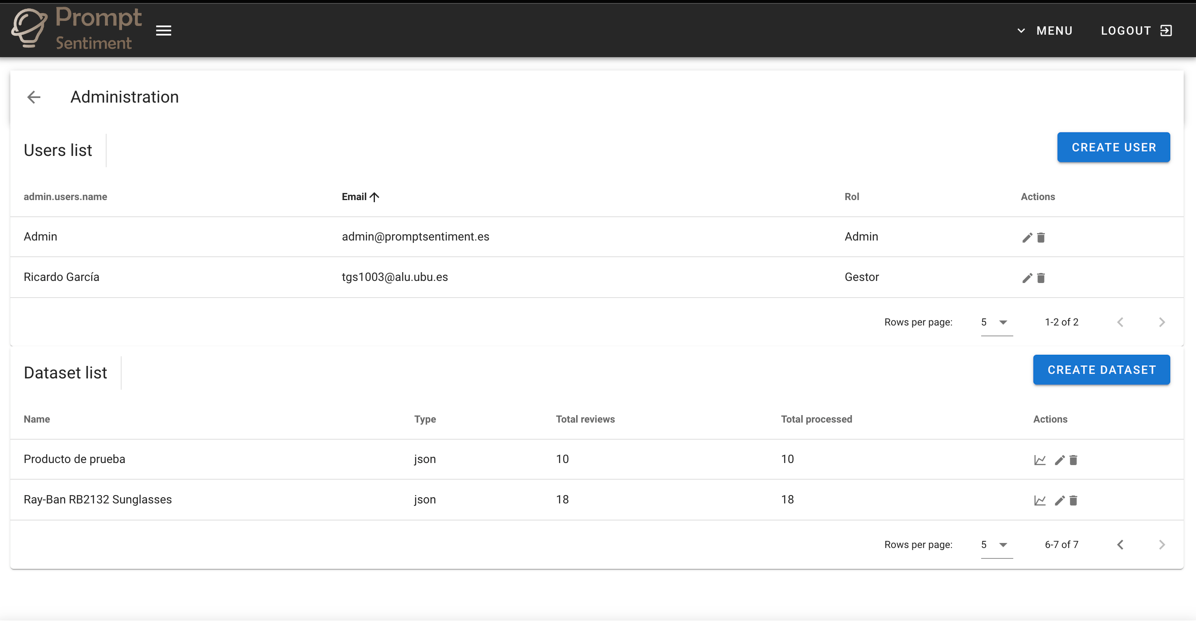
\includegraphics[width=12cm]{es/admin.png}}
\vspace{20pt}

\subsection{Usuarios}

Para crear un usuario pulsamos en el botón ``Nuevo usuario''

\vspace{20pt}
\centerline{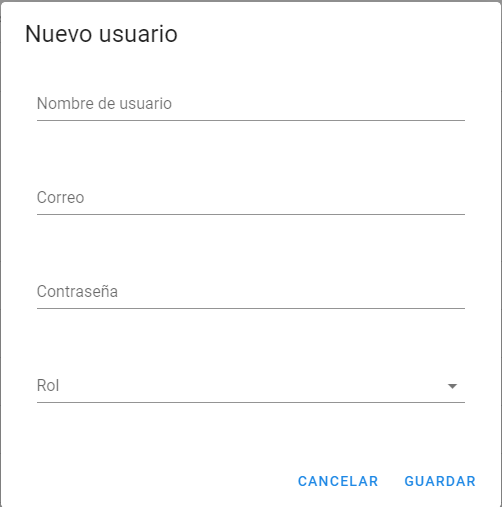
\includegraphics[width=6cm]{es/nuevo_usuario.png}}
\vspace{20pt}

Hay que rellenar los datos y pulsar en Aceptar.

Para borrar un usuario hay que pulsar en el icono de la papelera correspondiente al usuario que queremos borrar.
La aplicación pedirá confirmación:

\vspace{20pt}
\centerline{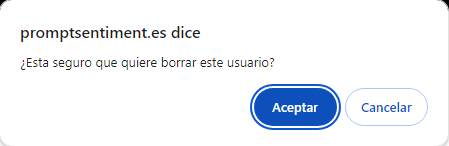
\includegraphics[width=8cm]{es/borrar_usuario.png}}
\vspace{20pt}

Para modificar los datos de un usuario hay que pulsar en el icono del lápiz.


\subsection{Conjuntos de datos}
Al igual que con los usuarios, desde la pantalla de administración se pueden administrar los conjuntos de datos.
En la versión actual de la aplicación sólo se pueden dar de alta desde de la pantalla de administración conjuntos de datos de tipo ``Hugging face''. \\Estos datasets están alojados en la página huggingface.com y necesitan un JSON de configuración.
Ejemplo:
\begin{verbatim}
    {         
        "name": "Amazon Shoe Reviews (test)",
        "type": "Hugging face",
        "path":"mesmalif/amazon-shoe-reviews",        
        "subset": "test",
        "mapping": {
            "review_text": "text",
            "review_headline": "review_headline",
            "stars": "labels",
            "review_id": "review_id",
            "review_date": "review_date"             
        },
        "correct_stars": 0,
        "date_format": "%Y-%m-%d"
    }
\end{verbatim}
Una vez configurado podemos cargarlo pulsado el icono 
\includegraphics[width=0.5cm]{upload.png}(cargar).
Nos preguntará el porcentaje a cargar:

\vspace{20pt}
\centerline{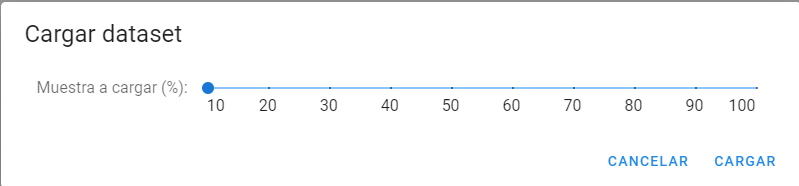
\includegraphics[width=8cm]{es/cargar_dataset.png}}
\vspace{20pt}

Cuando esté cargado se puede procesar pulsado el icono 
\includegraphics[width=0.3cm]{process.png}(procesar).
Al finalizar se pueden ver los resultados pulsando en el icono 
\includegraphics[width=0.5cm]{chart.png}(ver resultados)

\vspace{20pt}
\centerline{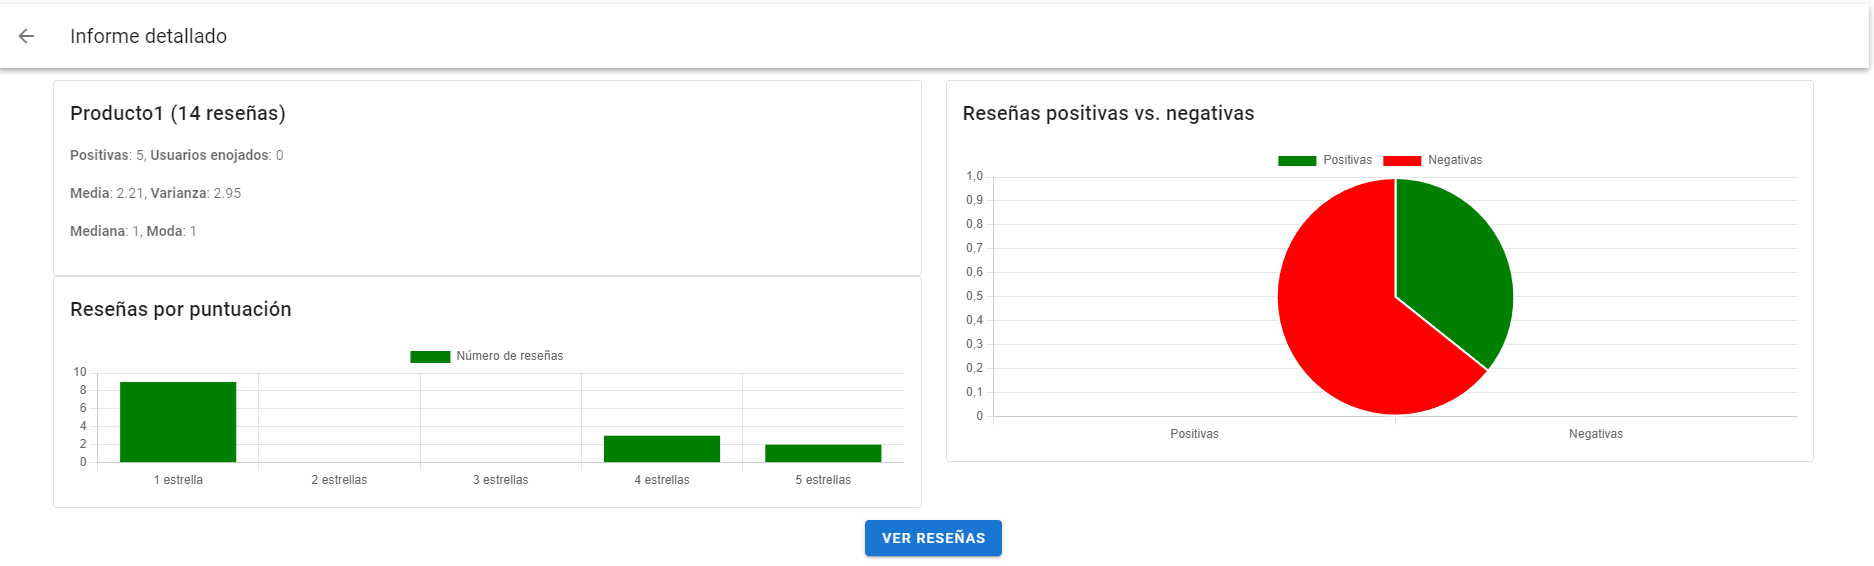
\includegraphics[width=14cm]{es/informe_detallado.png}}
\vspace{20pt}
\newpage
\section{Información}
En la pantalla de información podemos ver los datos de los autores, información de las herramientas utilizadas para su desarrollo así cómo una acceso al código de la aplicación en github.

\vspace{20pt}
\centerline{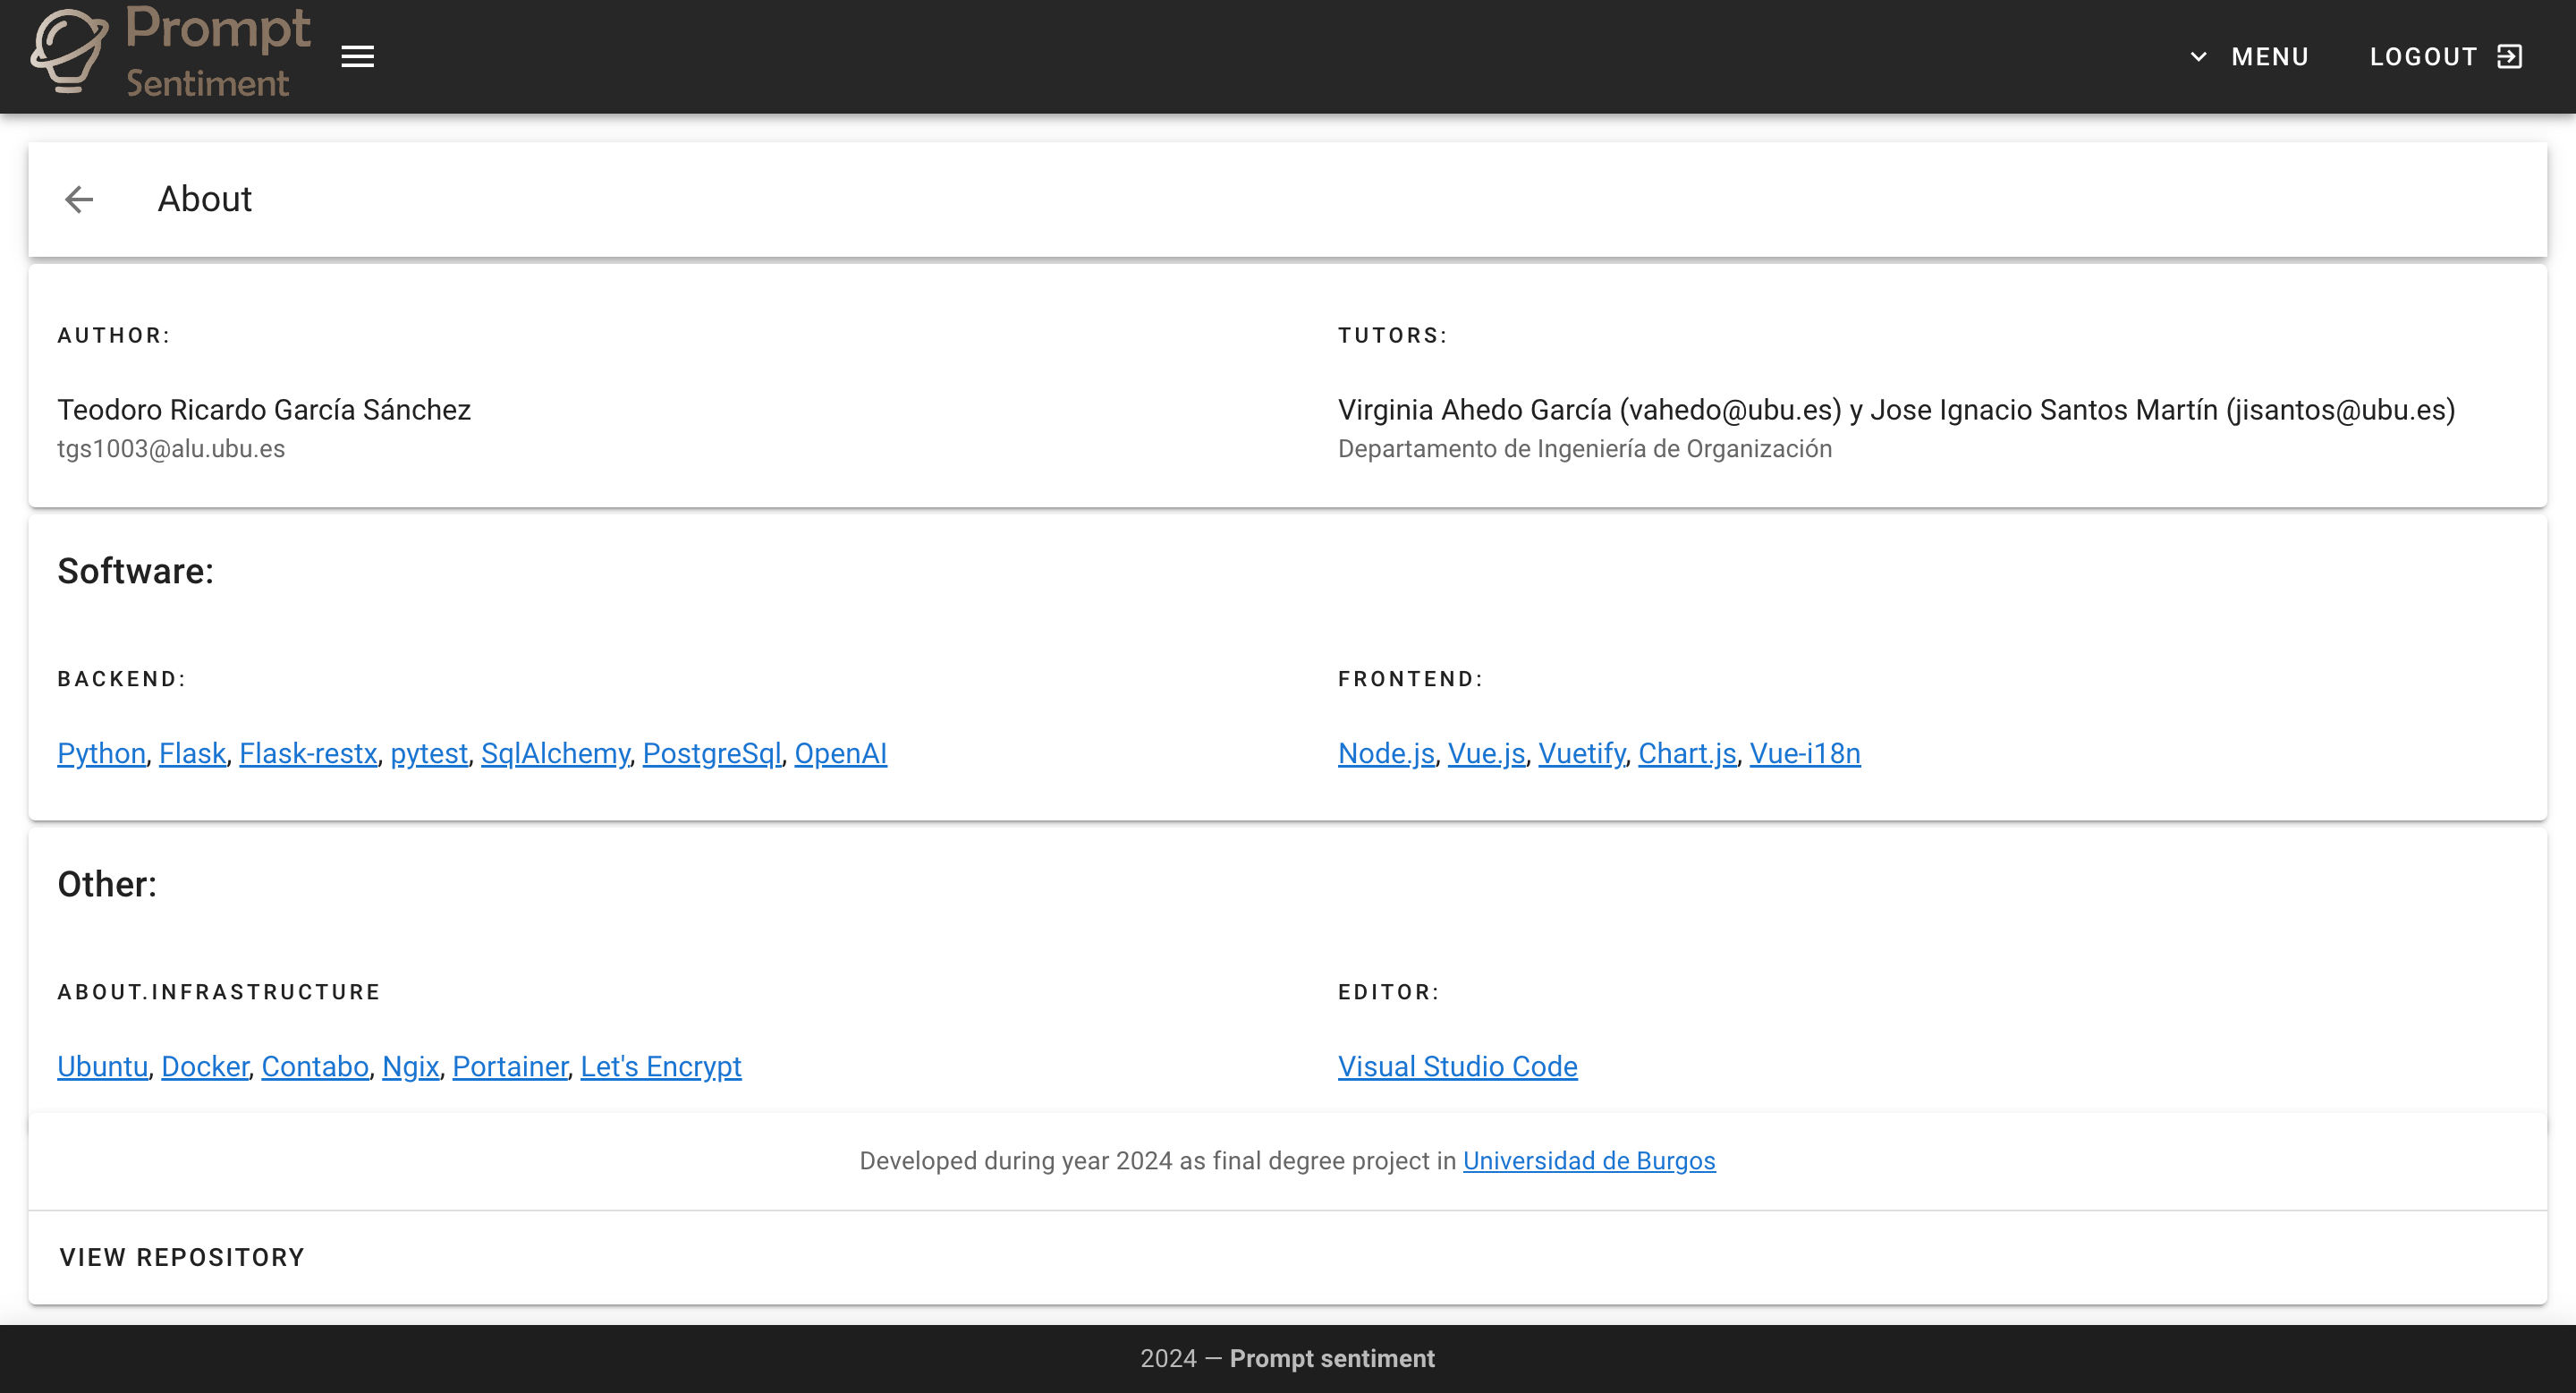
\includegraphics[width=14cm]{es/about.png}}
\vspace{20pt}

\end{document}
